\documentclass[a4paper, dvipsnames]{article}

\input ../header

\title{Chapitre 1 -- Les moteurs de recherche}

\author{}
\date{}

\begin{document}

\renewcommand{\contentsname}{}

\pagestyle{fancy}

\begin{tcolorbox}[colframe=blue!75, colback=blue!45, valign=center, height=1.5cm, top=5mm]
  \maketitle
\end{tcolorbox}

\tableofcontents

\vspace{1cm}

\thispagestyle{fancy}

Le Web contient des milliards de pages et il est constitué de millions de sites. Pour pouvoir \textbf{trouver de l'information} dans cette masse de données, les \textbf{moteurs de recherche} parcourent le Web pour créer un \textbf{index} à partir des contenus.

\vspace{1.5cm}

\section{Un bref historique}

\begin{activite}{frise chronologique}{}
  \begin{enumerate}
    \item Regarder la vidéo sur les moteurs de recherche dont le lien est donné sur Moodle.
    \item Télécharger les images du dossier \verb|Activité 1|.
    \item À l'aide d'un navigateur, se rendre sur la page web \url{http://www.frisechronos.fr/dojomain.htm} puis réaliser une frise chronologique sur les moteurs de recherche (attention, certains moteurs de recherche ne sont pas évoqués dans la vidéo).\\
      \textit{Remarque. -- Il est possible et fortement conseillé de sauvegarder régulièrement son travail. Chaque sauvegarde se fait sous la forme d'un fichier avec l'extension} \verb|bin|.
    \item 
      \begin{enumerate}
	\item Exporter la frise réalisée au format \verb|pdf|.
	\item Renommer le fichier obtenu au format \verb|NOM_Prénom_Classe.pdf| puis déposer la frise sur Moodle.
      \end{enumerate}
    \item 
      \begin{enumerate}
	\item Exporter la frise réalisée au format \verb|png|.
	\item Renommer le fichier obtenu au format \verb|NOM_Prénom_Classe.png| puis déposer la frise sur Moodle.
      \end{enumerate}
  \end{enumerate}
\end{activite}

\section{Qu'est-ce qu'un moteur de recherche ?}
Un moteur de recherche est un \textbf{service en ligne} permettant de trouver facilement une page sur le Web grâce à un ou plusieurs \textbf{mots-clés} renseignés dans un formulaire de recherche.

\begin{center}
  
\includegraphics[width=10cm]{ch_1_formulaire_moteur_de_recherche.png}
\end{center}

\medskip

\begin{activite}[breakable]{connaissez-vous des moteurs de recherche ?}{}
  \begin{enumerate}
    \item Donner le nom et l'adresse web de trois moteurs de recherche :

      \begin{center}
	\begin{tabular}{@{}ccc@{}}
	  \toprule
	& Moteur de recherche & Adresse web\\
	\midrule
	  1: & &\\
	  2: & &\\
	  3: & &\\
	  \bottomrule
	\end{tabular} 
      \end{center}
      \pagebreak
    \item Lire l'article suivant, puis répondre aux questions posées.

      \medskip
      \fbox{
	\begin{minipage}{\linewidth}
	  \begin{multicols}{2}
	    Et avant, comment faisait-on ? La question peut sembler étrange, presque incongrue tant Google a effacé, pour celles et ceux qui ont découvert Internet dans les années 1990, les souvenirs quasi traumatiques de la recherche « d’avant ». Plus personne ne veut revivre ça.

	    A l’époque, le choix même d’utiliser un moteur de recherche n’allait pas du tout de soi. La technologie phare, c’était l’annuaire : des centaines de liens classés en catégories, sous-catégories, et sous-sous-catégories. Mis à jour à la main, par des salariés de Yahoo! ou d’autres. On s’y plongeait un peu par hasard, en quête du bon site Web consacré au sujet sur lequel on voulait s’informer. C’était assez efficace pour trouver un forum de water-polo ou un site de recettes de gâteaux ; ça l’était beaucoup moins pour trouver une information précise.

	    Pour déceler ces dernières, il fallait effectivement passer par un moteur. Le processus était long et fastidieux : on entrait sa recherche, en tâtonnant. Comment parle-t-on à un moteur de recherche ? La question peut paraître triviale aujourd’hui, mais était loin d’être évidente. « Je cherche en quelle année a débuté la guerre du Vietnam » ne vous emmenait nulle part. « Guerre Vietnam » donnait de meilleurs résultats, mais n’était pas assez précis. On ajoutait, on enlevait des mots un peu au hasard. On comparait « début guerre Vietnam » avec « guerre Vietnam début », avant de se résoudre à tester « beginning Vietnam War ». Les opérateurs booléens, les fameux « + » et « – » permettant d’affiner sa recherche, étaient une technologie balbutiante introduite par AltaVista, et encore mystérieuse pour quasi tout le monde.
	  \end{multicols}
	\end{minipage}
      }
      \begin{flushright}
	\scriptsize
	Source : \url{https://www.lemonde.fr/pixels/article/2018/09/04/avant-google-comment-faisait-on_5350028_4408996.html}
      \end{flushright}

      \begin{enumerate}
	\item Avant les moteurs de recherche, quel type de service utilisait-on pour trouver une page ou une information sur le Web ?\rep{2}
	\item Quelles sont les difficultés rencontrées par les utilisateurs avec ce type de service ?\rep{2}
	\item Comment fallait-il procéder pour obtenir des informations précises avec les premiers moteurs de recherche ?\rep{2}
      \end{enumerate}
  \end{enumerate} 
\end{activite}

%\activite[Un peu de Python]
%
%On considère le programme suivant :
%
%\begin{minted}[linenos,frame=single,xleftmargin=1cm,xrightmargin=1cm]{python}
%def formulaire_recherche():
%    recherche = input("Que recherchez-vous ?")
%    print("Vous cherchez :", recherche)
%\end{minted}
%
%\begin{enumerate}
%  \item 
%    \begin{enumerate}
%      \item Essayer ce \og{}programme\fg{} en écrivant \mintinline{python}{formulaire_recherche()}.
%      \item Donner une description des mots-clés \mintinline{python}{def}, \mintinline{python}{input} et \mintinline{python}{print} du langage Python.\rep{3}
%    \end{enumerate}
%  \item 
%    \begin{enumerate}
%      \item Remplacer la dernière ligne du programme par \mintinline{python}{print("Vous cherchez :" + recherche)}.
%      \item Essayer à nouveau le programme puis expliquer la différence entre les instructions :
%	\begin{minted}[frame=single,xleftmargin=2cm,xrightmargin=2cm]{python}
%print("Vous cherchez :", recherche)
%	\end{minted}
%	et :
%	\begin{minted}[frame=single,xleftmargin=2cm,xrightmargin=2cm]{python}
%print("Vous cherchez :" + recherche)
%	\end{minted}
%	\dotfill\rep{2}
%    \end{enumerate}
%  \item     
%    \begin{enumerate}
%      \item Ajouter à la dernière ligne du (premier) programme les deux lignes suivantes :
%    \begin{minted}[frame=single,xleftmargin=2cm,xrightmargin=2cm]{python}
%mots = recherche.split(" ")
%print("Les mots-clés sont :", mots)
%    \end{minted}
%  \item Essayer le programme en entrant la recherche \mintinline{python}{langage programmation Python} puis donner la signification de l'instruction \mintinline{python}{recherche.split(" ")}.\rep{3}
%    \end{enumerate}
%\end{enumerate}
%
\section{Comment fonctionne un moteur de recherche ?}

Le fonctionnement d’un moteur de recherche se décompose en trois processus principaux :
\begin{enumerate}
  \item \textbf{L’exploration} : le web est exploré par un robot, appelé crawler ou spider, qui suit tous les liens qu’il trouve et qui récupère les ressources jugées intéressantes. L’exploration est lancée depuis une ressource pivot, comme une page d’annuaire web.
  \item \textbf{L’indexation} des ressources récupérées consiste à extraire les mots considérés comme significatifs. Les mots extraits sont enregistrés dans une base de données organisée comme un
    gigantesque dictionnaire appelé index.
  \item \textbf{La recherche} correspond au formulaire moteur. Un algorithme est appliqué pour identifier les ressources de l’index qui correspondent le mieux aux mots contenus dans la requête. Les résultats de la recherche sont ensuite affichés par ordre de pertinence.
\end{enumerate}

\medskip

\begin{activite}[breakable]{faire une recherche pertinente}{}
  \begin{enumerate}
    \item Ouvrir la page \url{https://www.google.com} à l'aide d'un navigateur web.
    \item Les mots-clés d'une recherche :
      \begin{enumerate}
	\item Effectuer la recherche suivante :
	  \begin{center}
	    \verb|Tout savoir sur le réchauffement climatique en France|
	  \end{center}
	  Combien de résultats obtient-on ? \dotfill
	\item Effectuer la recherche suivante :
	  \begin{center}
	    \verb|Réchauffement climatique en France|
	  \end{center}
	  Combien de résultats obtient-on ? \dotfill
	\item Effectuer la recherche suivante :
	  \begin{center}
	    \verb|Réchauffement climatique France|
	  \end{center}
	  Combien de résultats obtient-on ? \dotfill
	\item Donner une explication sur la différence du nombre de résultats obtenus pour les recherches précédentes.\rep{2}
      \end{enumerate}
    \item Affiner ses recherches :
      \begin{enumerate}
	\item Effectuer la recherche suivante :
	  \begin{center}
	    \verb|réchauffement climatique "en France"|
	  \end{center}
	  Combien de résultats obtient-on ? \dotfill
	\item Effectuer la recherche suivante :
	  \begin{center}
	    \verb|"réchauffement climatique" "en France"|
	  \end{center}
	  Combien de résultats obtient-on ? \dotfill
	\item Donner une explication sur la différence du nombre de résultats obtenus pour les recherches précédentes.\rep{2}
	\item Effectuer la recherche suivante :
	  \begin{center}
	    \verb|"réchauffement climatique" "en France" site:gov|
	  \end{center}
	  Combien de résultats obtient-on ? \dotfill\\
	  Quelle est la particularité des liens affichés dans les résultats de la recherche ?\rep{1}
	\item Effectuer la recherche suivante :
	  \begin{center}
	    \verb|filetype:pdf "réchauffement climatique" "en France" site:gov|
	  \end{center}
	  Combien de résultats obtient-on ? \dotfill\\
	  Quelle est la particularité des liens affichés dans les résultats de la recherche ?\rep{1}
      \end{enumerate}
    \item 
      \begin{enumerate}
	\item Pour obtenir des informations sur les sites \verb|.edu| sur les \verb|moteurs de recherche|, quelle requête peut-on écrire ?\rep{2}
	\item Pour obtenir des informations sur le site web de la \verb|cnil.fr| en format \verb|pdf| sur les \verb|moteurs de recherche| en y excluant les résultats parlant de \verb|google|, quelle requête peut-on écrire ?\rep{2}
      \end{enumerate}
  \end{enumerate} 
\end{activite}

\section{Les résultats d'un moteur de recherche}

Les moteurs de recherche ont développé des méthodes de tri automatiques des résultats. Dans la pratique aucune méthode de tri n’est parfaite mais cette variété offre à l’utilisateur la possibilité de traquer l’information de différentes manières et augmente donc ses chances d’améliorer ses recherches.

\medskip

Si on ne trouve pas ce que l’on cherche dans les toutes premières pages de résultats, il faut reformuler la question. 

\medskip

On peut considérer trois grandes méthodes de tris :

\begin{enumerate}
  \item \textbf{Le tri par pertinence} : les résultats d’une requête sont affichés selon un ordre basé sur le poids d’un mot et la fréquence d’apparition du mot dans un document.
  \item \textbf{Le tri par popularité} : les résultats d’une requête sont affichés selon un ordre basé sur le nombre de liens entrant et l’audience du document.
  \item \textbf{Le tri par catégorie} : les résultats d’une requête sont affichés selon un ordre basé sur le sujet, le type, la source et la langue du document.
\end{enumerate}

\medskip

\begin{activite}{distinguer les résultats d'une recherche}{}
  On tombe sur les deux liens ci-dessous dans les résultats d'une recherche :

  \begin{center}
    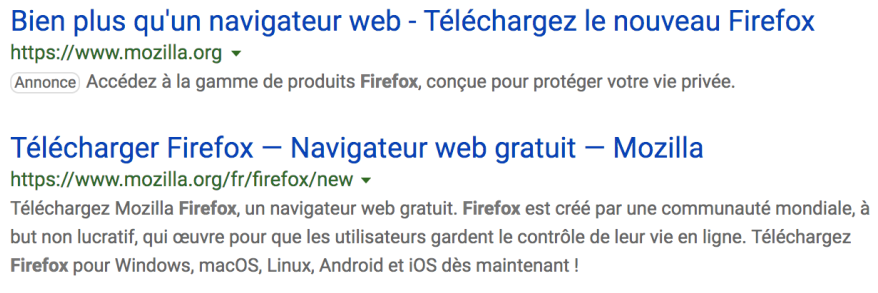
\includegraphics[width=12cm]{ch_1_recherche_firefox.png}
  \end{center}

  Quelle différence y a-t-il entre ces deux résultats ?\rep{2}
\end{activite}


\end{document}
